\documentclass[11pt, letter]{amsart}


\usepackage[margin=1in]{geometry}
\usepackage{amsthm}
\usepackage{amsmath}
\usepackage{amssymb}
\usepackage{enumerate}
\usepackage[inline]{enumitem}
\usepackage{graphicx}

\newtheorem*{theorem*}{Theorem}
\newtheorem*{lemma*}{Lemma}
\theoremstyle{definition}
\newtheorem{problem}{Problem}[]
\newtheorem{exercise}{Exercise}[]
\newtheorem*{definition*}{Definition}

\title{Final Exam Solutions}
\author{Sean Eva}

\begin{document}

\maketitle

\begin{exercise}
\end{exercise}
\begin{enumerate}
    \item 

    We are going to note that a subset of a metric space is compact if and only if it is complete and totally bounded. Since $\psi(\mathbb{S}^1)$ is a closed and bounded subset of $\mathbb{R}^2$, it is complete and totally bounded. Therefore, $\psi(\mathbb{S}^1)$ is compact as desired.

    \item 

    A compact subset of a metric space is closed by definition. Thus, $\psi(\mathbb{S}^1)$ is closed as desired.

    \item 

    \begin{enumerate}
        \item 

        Since $\phi$ is a homeomorphism, it is continuous and has a continuous inverse. Thus, $\phi(I)$ is an open subset of $\mathbb{R}$, and since $y\in I \Rightarrow y\in \phi(I)$ as desired.

        \item 

        Since $I$ is an open subset of $\mathbb{S}^1$ and $y$ is arbitrary, it follows that $\mathbb{S}^1$ is an open subset of $\mathbb{R}$ as desired.
        
    \end{enumerate}

    \item 

    Since $\mathbb{S}^1$ is non-empty and open in $\mathbb{R}$, it must have a non-empty interior. Therefore, there exists points in $\mathbb{S}^1$ arbitrarily close to another point in $\mathbb{S}^1$. That is to say that $\mathbb{S}^1$ is dense in $\mathbb{R}$.

    \item 

    The contradiction follows from the fact that a connected, dense subset of $\mathbb{R}$ must be uncountable. However, since $\mathbb{S}^1$ is a 1-dimensional manifold and thus has a countable basis of open sets. Therefore, $\mathbb{S}^1$ cannot be dense in $\mathbb{R}$. Thus, the assumption that $\mathbb{S}^1$ can be embedded in $\mathbb{R}$ leads to a contradiction, and so such an embedding does not exist.
    
\end{enumerate}


\begin{exercise}
\end{exercise}
\begin{enumerate}
    \item 

    Let us define a homotopy between $D$ and $\{0\}$ as $H(D, t) = (1 - t)D + t\{0\}$ for $t\in [0, 1]$ where $H(D, 0) = D, H(D, 1) = \{0\}$. It is simple to see that $H$ is well-defined and is an equivalence relation. Therefore we find that $D \simeq \{0\}$ and are homotopically equivalent as desired.

    \item 

    The fundamental group of $D$ based at any point $\pi_1(D, a)$ is just the identity element, i.e. the trivial group. It is easy to see that $D \simeq \{a\}$ for arbitrary constant $a$. Any two points can shrink to each other to the identity element in any simply connected space that is loop based to a point. For D, every loop can be shrunk to a single loop. Therefore, we find that $\pi_1(D, a) = \{e\}$ where $e$ is the identity element, representing the trivial group.

    \item 

    \begin{enumerate}
        \item 

        First, we are going to note that $f(z) = \frac{z}{|z|} = \{(r\cos(2t\pi), r\sin(2t\pi): r\in (0, 1], t\in [0, 1]\}$.To show that there is a homotopy between $X$ and $\mathbb{S}^1$ we are going to define a homotopy $H: X \times I \rightarrow \mathbb{S}^1$ as $H(X, T) = (1 - T)f_0 + Tf_1(z)$ where $H(X, 0) = f_0 = (\cos(0), \sin(0) = (1, 0)$ and $H(X, 1) = f_1 = (\cos(2\pi), \sin(2\pi)) = (0, 1).$ This implies then that $H$ sends all the points of $X$ to $\mathbb{S}^1$ and $H$ is an equivalence relation. Therefore, we know that $f: X \rightarrow \mathbb{S}^1$ is an equivalence of homotopy.

        \item 

        Since we know that $X \simeq \mathbb{S}^1$ we also know that $\pi_1(\mathbb{S}^1, x_0) = \mathbb{Z}$. Therefore, we know that if $x_0 = 1$, then $\pi_1(X, 1) = \mathbb{Z}$.

        \item 

        $X$ is like a disc with a hole in the center (Figure \ref{fig:X}). A non-trivial element of $\pi_1(X, 1) = \{(\cos(2\pi ns), \sin(2\pi ns): s\in \mathbb{R}, n\in \mathbb{Z}\}$ is $(\cos(2\pi n), \sin(2\pi n))$ which would just be the outer boundary.
        
    \end{enumerate}
\end{enumerate}

\begin{center}
\begin{figure}
    \centering
    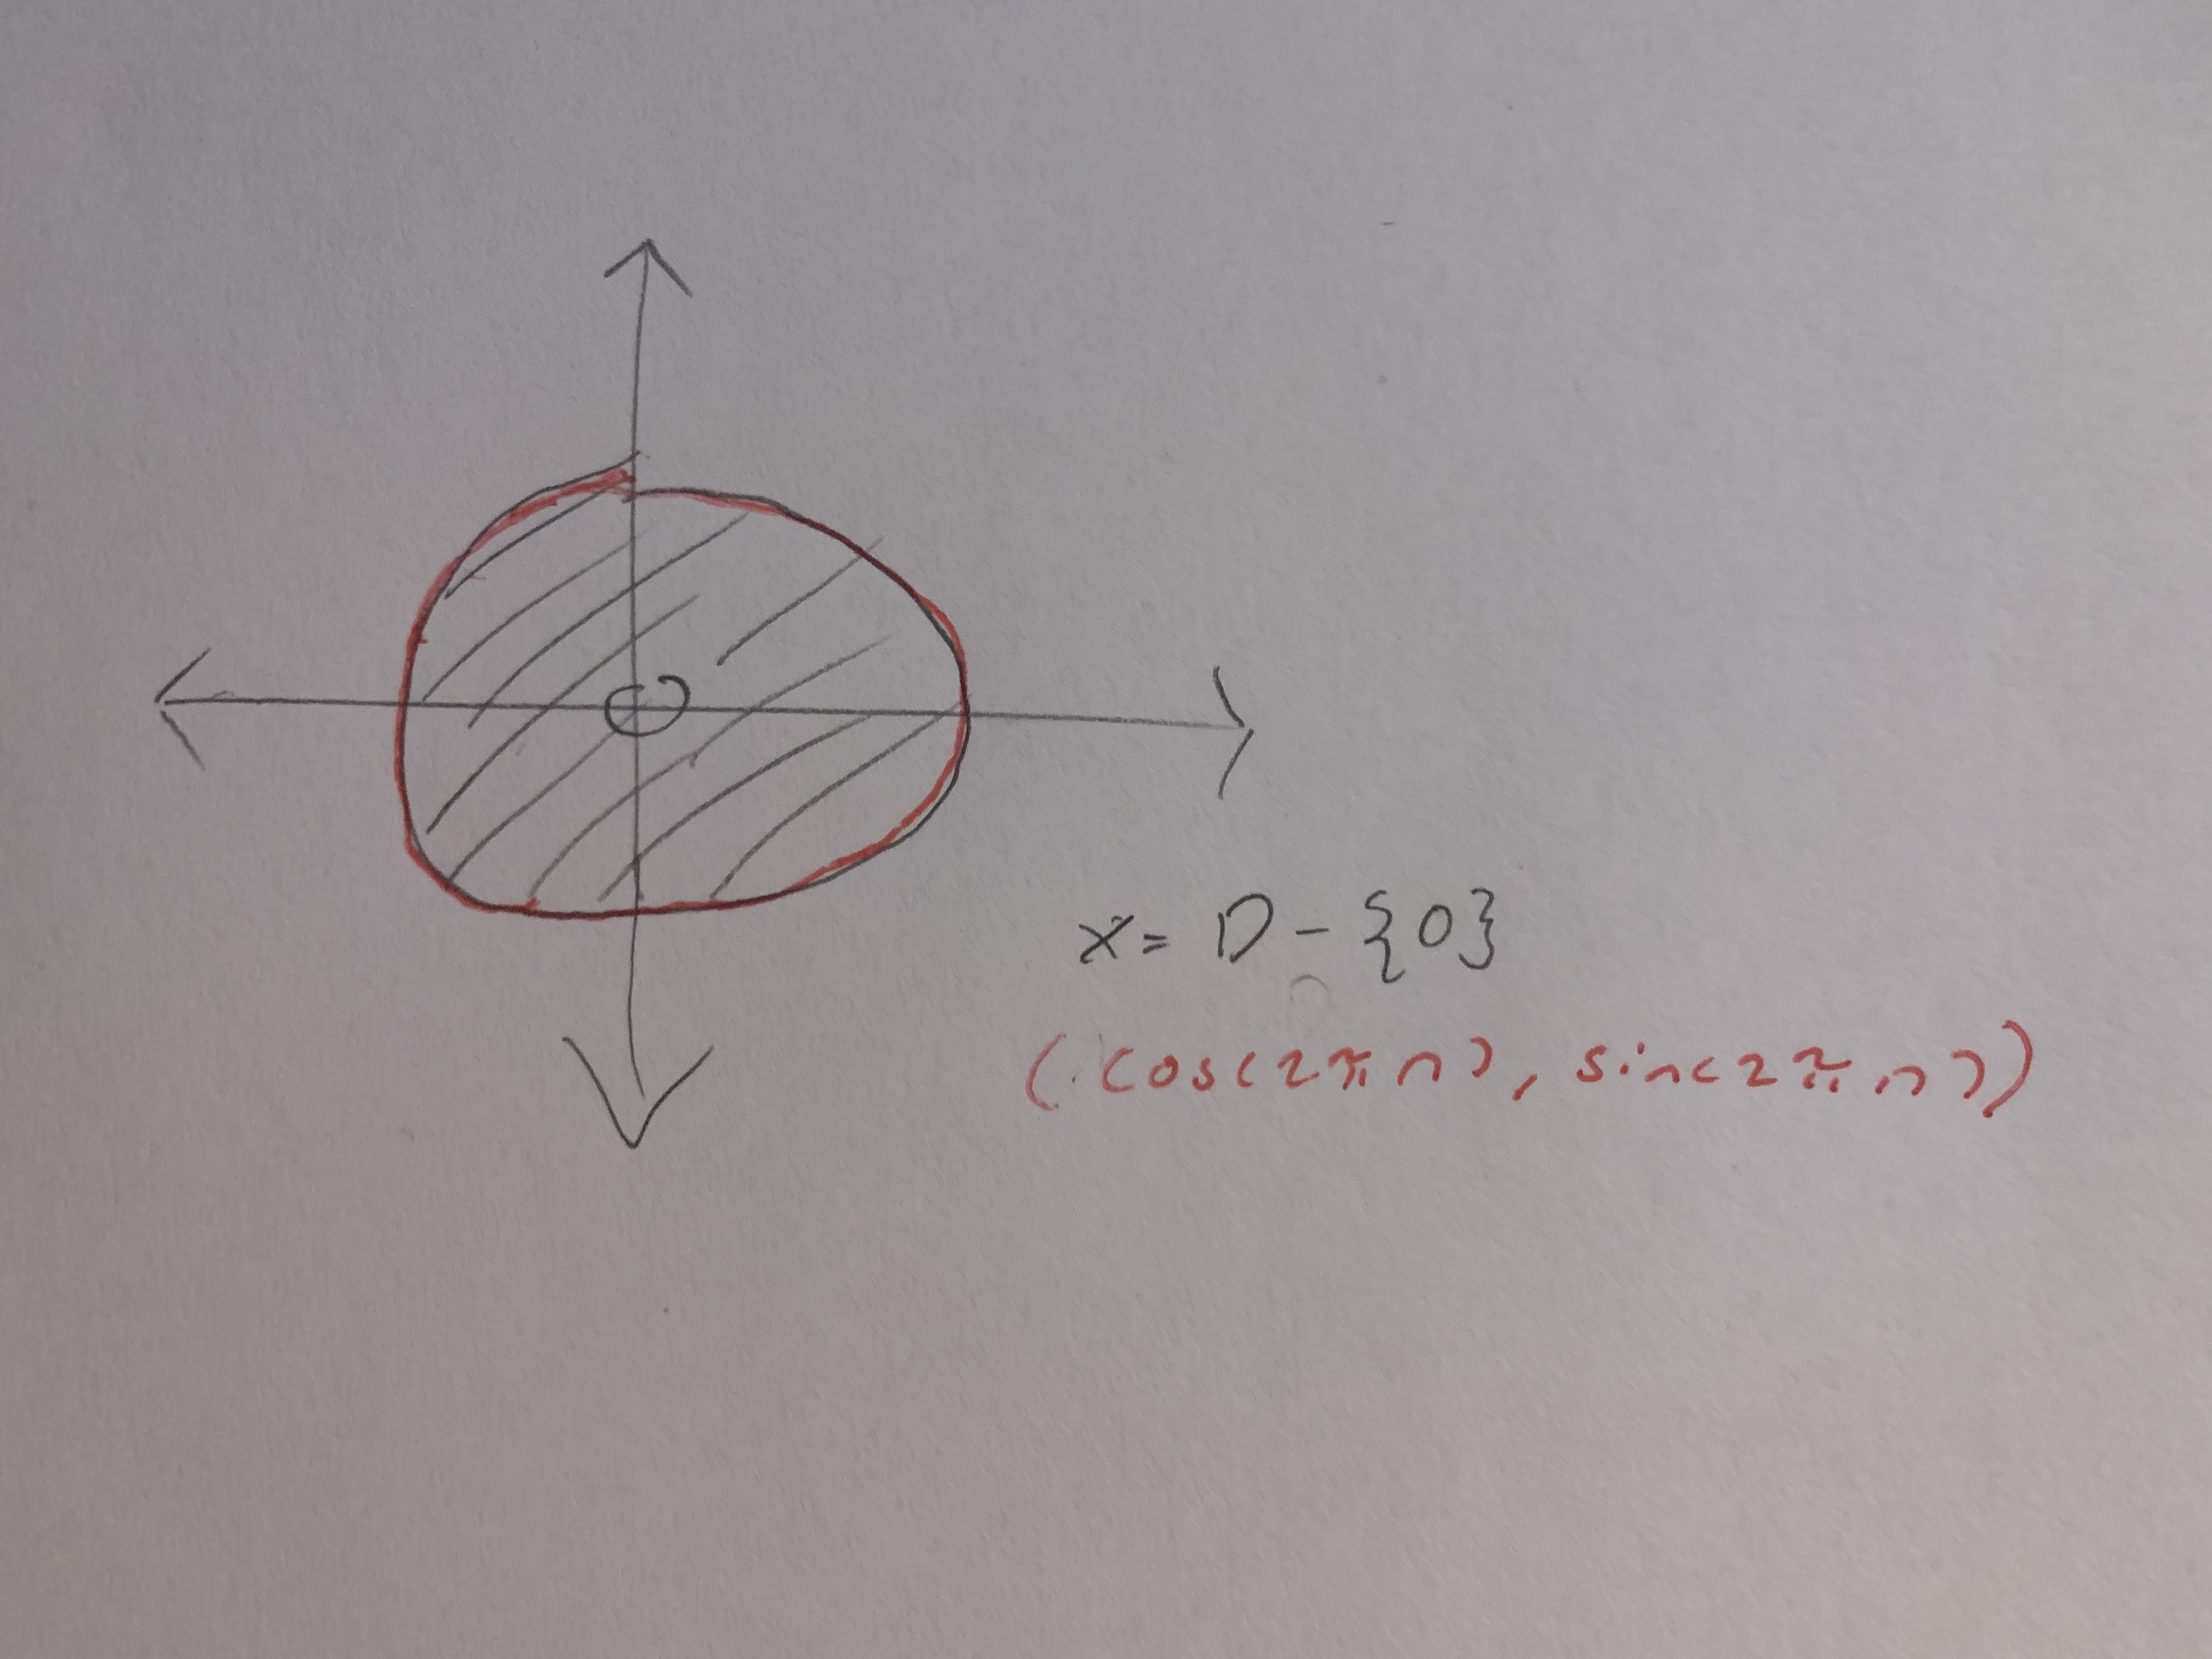
\includegraphics[scale=0.1]{Drawing of X.jpg}
    \caption{Drawing of $X$ with a non-trivial element of $\pi_1(X, 1)$}
    \label{fig:X}
\end{figure}
\end{center}


\end{document}
